% ----------------------------------------------------------------------
% Configurar a classe do documento
% ----------------------------------------------------------------------
\documentclass[11pt]{article}

% ----------------------------------------------------------------------
% Definir packages externos, língua, margens, tipos de letra, novos 
% comandos e cores
% ----------------------------------------------------------------------
\usepackage[utf8]{inputenc} % Codificação utilizada
\usepackage[portuguese]{babel} % Idioma de escrita
\usepackage[normalem]{ulem}

\usepackage[bottom]{footmisc}

\usepackage{listings}
\usepackage{color}
\usepackage{eurosym}

\usepackage{verbatim}
\usepackage{gensymb}
\usepackage[export]{adjustbox} % Alinhar imagens
\usepackage{amsmath} % Comandos extra para escrita matemática
\usepackage{amssymb} % Símbolos matemáticos
\usepackage{anysize} % Personalizar as margens
    \marginsize{1.5cm}{1.5cm}{1.5cm}{1.5cm} % {esquerda}{direita}{cima}{baixo}
\usepackage{appendix} % Apêndices
\usepackage{cancel} % Cancelar expressões
\usepackage{caption} % Legendas
    \DeclareCaptionFont{newfont}{\fontfamily{cmss}\selectfont}
    \captionsetup{labelfont={bf, newfont}}
\usepackage{cite} % Citações, tipo [1 - 3]
\usepackage{color} % Colorir texto
\usepackage{fancyhdr} % Cabeçalho e rodapé
    \pagestyle{fancy}
    \fancyhf{}
    \fancyhead[L]{
\includegraphics[width=2cm]{Imagens/IST}} % Esquerda do cabeçalho
    \fancyhead[R]{\footnotesize\fontfamily{cmss}\selectfont Sistemas Eletrónicos} % Direita do cabeçalho
    \fancyfoot[L]{\footnotesize\fontfamily{cmss}\selectfont LAB 3 - $\mu$Oscilloscope} % Esquerda do rodapé
    \fancyfoot[C]{\thepage} % Centro do rodapé
    \fancyfoot[R]{\footnotesize\fontfamily{cmss}\selectfont LEEC} % Direita do rodapé
    \renewcommand{\footrulewidth}{0.4pt} % Régua do rodapé
\usepackage{float} % Utilizar o especificador [H] nas figuras
\usepackage{graphicx} % Imagens em LaTeX
\usepackage[colorlinks = true, plainpages = true, linkcolor = istblue, urlcolor = istblue, citecolor = istblue, anchorcolor = istblue]{hyperref}
\usepackage{indentfirst} % Primeiro parágrafo
\usepackage{siunitx} % Unidades SI
\usepackage{subcaption} % Subfiguras
\usepackage{titlesec} % Tipo de letra
    \titleformat{\section}{\fontfamily{cmss}\selectfont\Large\bfseries}{\thesection}{1em}{}
    \titleformat{\subsection}{\fontfamily{cmss}\selectfont\large\bfseries}{\thesubsection}{1em}{}
    \titleformat{\subsubsection}{\fontfamily{cmss}\selectfont\normalsize\bfseries}{\thesubsubsection}{1em}{}
    \fancyfoot[C]{\fontfamily{cmss}\selectfont\thepage}

\usepackage{float}
\usepackage{afterpage}
\usepackage{multirow} % para mesclar células verticalmente
\usepackage{array} % para ajustar o espaçamento das colunas
\usepackage{makecell}
\usepackage{float} % para definir o posicionamento da tabela
\usepackage{acronym}
\usepackage{xltabular}
\usepackage{colortbl} % Adicione o pacote colortbl para cores nas células
\usepackage{xcolor}
\usepackage{cleveref}
\usepackage{soul}

% Novos e renovar comandos
\newcommand{\sen}{\operatorname{\sen}} % Definição da função seno
\newcommand{\HRule}{\rule{\linewidth}{0.5mm}} % Definição de uma régua
\renewcommand{\appendixpagename}{\LARGE \fontfamily{cmss}\selectfont Apêndices}
\renewcommand{\appendixtocname}{Apêndices}
\renewcommand{\lstlistingname}{Código}

% Cores
\definecolor{lightblue}{rgb}{0.678, 0.847, 0.902} % Definindo uma nova cor de azul claro
\definecolor{istblue}{RGB}{3, 171, 230}
\definecolor{dkgreen}{rgb}{0,0.6,0}
\definecolor{gray}{rgb}{0.5,0.5,0.5}

\sethlcolor{istblue} % Set highlight color to blue

\usepackage{lipsum}

\definecolor{backcolour}{rgb}{0.95,0.95,0.92}
\definecolor{codegreen}{rgb}{0,0.5,0}
\definecolor{codepurple}{rgb}{0.5,0,0.5}
\definecolor{codeblue}{rgb}{0,0,0.7}
\definecolor{codegray}{rgb}{0.5,0.5,0.5}

\lstdefinestyle{mystyle}{
    backgroundcolor=\color{backcolour},   
    commentstyle=\color{codegreen},
    keywordstyle=\color{codeblue},
    numberstyle=\tiny\color{codepurple},
    stringstyle=\color{codepurple},
    basicstyle=\ttfamily\footnotesize,
    breakatwhitespace=false,         
    breaklines=true,                 
    captionpos=b,                    
    keepspaces=true,                 
    numbers=left,                    
    numbersep=5pt,                  
    showspaces=false,                
    showstringspaces=false,
    showtabs=false,                  
    tabsize=2,
    language=Python % Change this line to Python
}

\lstdefinestyle{mystyle_complete_code}{
    backgroundcolor=\color{backcolour},   
    commentstyle=\color{codegreen},
    keywordstyle=\color{codeblue},
    numberstyle=\tiny\color{codepurple},
    stringstyle=\color{codepurple},
    basicstyle=\ttfamily\tiny, % Change to \tiny for the smallest font size
    breakatwhitespace=false,         
    breaklines=true,                 
    captionpos=b,                    
    keepspaces=true,                 
    numbers=left,                    
    numbersep=5pt,                  
    showspaces=false,                
    showstringspaces=false,
    showtabs=false,                  
    tabsize=2,
    language=Python % Change this line to Python
}

\lstset{style=mystyle_complete_code}

%%%%%%%%%%%%%%%%%%%%%%%%%%%%%%%%%%%%%%%%%%%%%%%%%%%%%%%%%%%%%%%%%%%%%%%%
%                               Documento                              %
%%%%%%%%%%%%%%%%%%%%%%%%%%%%%%%%%%%%%%%%%%%%%%%%%%%%%%%%%%%%%%%%%%%%%%%%
\begin{document}

% ----------------------------------------------------------------------
% Capa
% ----------------------------------------------------------------------
\begin{titlepage}

\begin{picture}(0,0)
  \put(-35,5){
\includegraphics[width=6cm]{Imagens/IST}}
\end{picture}

\center

\large Instituto Superior Técnico\\[1 cm] 

\large Licenciatura em Engenharia Eletrotécnica e de Computadores\\[2 cm] 
\LARGE \textbf{Sistemas Eletrónicos}\\[1 cm] 
\large 2023/2024 - Segundo Semestre (3º Período)\\[2 cm]
\LARGE \underline{LAB 3 - $\mu$Oscilloscope}\\[1 cm]
\LARGE {Osciloscópio através de um sistema embebido}\\[1 cm]
\large \underline{Grupo 50}

\vspace{1cm}

\begin{center}
    \begin{minipage}{0.5\textwidth}
        \begin{flushleft}
            \normalsize António Vasco Morais de Carvalho (102643)\\
            \normalsize Catarina Andreia Duarte Caramalho  (102644)\\
            \normalsize João Pedro Mendes Pinheiro (102709)
        \end{flushleft}
    \end{minipage}%
    \begin{minipage}{0.5\textwidth}
        \begin{flushright}
            \href{mailto:antonio.v.morais.c@tecnico.ulisboa.pt}{\normalsize\texttt{\textcolor{istblue}{antonio.v.morais.c@tecnico.ulisboa.pt}}}\\
            \href{mailto:catarina.caramalho@tecnico.ulisboa.pt}{\normalsize\texttt{\textcolor{istblue}{catarina.caramalho@tecnico.ulisboa.pt}}}\\
            \href{mailto:joaoppinheiro@tecnico.ulisboa.pt}{\normalsize\texttt{\textcolor{istblue}{joaoppinheiro@tecnico.ulisboa.pt}}}
        \end{flushright}
    \end{minipage}
\end{center}

\vspace{1cm}

Auto-avaliação: 18/20

\vspace{1.5 cm}

Dia da semana: Terça-feira

Turno: 10:00 - 11:30
\vspace{1.5 cm}

\underline{Docente: Diogo Miguel Caetano} \\

\end{titlepage}

\setcounter{page}{0}

% ----------------------------------------------------------------------
%                                 Conteúdo
% ----------------------------------------------------------------------
\thispagestyle{empty} % Remover cabeçalho e rodapé da página do índice
\tableofcontents 

\newpage

% ----------------------------------------------------------------------
%                              Desenvolvimento
% ----------------------------------------------------------------------
\section{Introdução}\label{sec:Introdução}
    % No presente trabalho laboratorial, foi desenvolvido um osciloscópio através de um sistema embebido, com o objetivo de criar uma ferramenta de medição e análise de sinais eletrónicos. Os testes laboratoriais visam verificar a apresentação gráfica do programa, explorar as escalas de medição, obter leituras para diferentes tensões, realizar a calibração do sistema e validar o desempenho do osciloscópio com diferentes formas de onda. 

No presente trabalho de laboratório pretende estudar-se sistemas embebidos, ainda que superficialmente, os quais correspondem a uma combinação de um \textit{hardware} computacional e um \textit{software} projetado para uma função específica. Para tal utilizar-se-á um módulo IoT composto por uma placa micro-controladora com diversas funcionalidades e interfaces e capaz de funcionar como um osciloscópio com um \textit{software} desenvolvido para tal. Com isto, definem-se os objetivos do trabalho: Aprendizagem do circuito de \textit{hardware} base para a realização do trabalho; Desenvolvimento do \textit{software} para implementação do $\mu$Oscilloscope; Teste e ajuste do \textit{software}; Calibração do $\mu$Oscilloscope.

Primeiramente, explica-se o \nameref{sec:Programa desenvolvido} pelo grupo (\texttt{main.py}) com o qual se fizeram \nameref{sec:Testes no simulador} previamente às aulas de laboratório. De seguida apresentam-se os \nameref{sec:Testes no laboratório} onde se esperam ver incongruências na representação dos sinais com a ausência de calibração, mas que após um ajuste experimental, isto é, uma calibração experimental, se espera que essas incongruências sejam erradicadas quase totalmente (sempre sujeito a imperfeições experimentais).

\section{Programa desenvolvido}\label{sec:Programa desenvolvido}
    De modo a cumprir as funções especificadas no enunciado, tomaram-se como base os \textit{scripts} fornecidos pelos docentes (\texttt{main\_exemplo\_1.py} e \texttt{main\_exemplo\_2.py}) para o desenvolvimento do programa \texttt{main.py}.

Nesta secção serão apresentadas porções do código consideradas mais importantes para a sua perceção do ponto de vista do leitor. Para erradicar quaisquer dúvidas, o código completo encontra-se no \autoref{ap:Ficheiro de código desenvolvido completo} e devidamente comentado. \newline

Primeiramente reconheçam-se as variáveis globais utilizadas, com especial atenção para as variáveis das linhas \texttt{15}, \texttt{16}, \texttt{21} e \texttt{22} que correspondem à informação de um sinal em pixeis dos dois eixos (para a representação no \textit{display}) e aos índices dos vetores das escalas para efetuar a mudança de escala consoante o botão premido (no ciclo principal do programa incrementam-se estes índices ao receber \textit{input} dos botões respetivos). Notemos ainda a variável da linha \texttt{31} que, quando a \texttt{True}, possibilita a mudança de escalas e permanecendo na representação do espetro, mudando o seu valor para \texttt{False} aquando da representação no domínio do tempo.

\lstinputlisting[language=Python, label={lst:variaveis}, firstline=8, lastline=32,firstnumber=8]{codigo_completo.py}

O programa principal começa por executar \texttt{reset\_display()} e \texttt{read\_and\_calculate()}. Esta última apresentada abaixo, calcula as tensões a partir dos pontos recolhidos do ADC, determina parte do conjunto de medidas a enviar por email (valor eficaz é calculado à parte com \texttt{calculate\_rms\_value()}) e converte as tensões em pixeis para representar o sinal no \textit{display} através de \texttt{draw\_normal\_plot()}.

\lstinputlisting[language=Python, label={lst:readandcalculuate}, firstline=59, lastline=97,firstnumber=59]{codigo_completo.py}

De seguida inicia-se o ciclo principal do programa onde se espera pelo acionamento de alguma das funções pedidas para desenvolver, através da pressão de um botão por parte do utilizador. Por motivos de extensividade, esse ciclo não é aqui apresentado, mas pode ser consultado em detalhe no \autoref{ap:Ficheiro de código desenvolvido completo}. \newline

Ao pressionar o \textbf{Botão 1}: \uline{Clique rápido -} estamos no domínio do tempo e as escalas voltam ao padrão (modificando as variáveis \texttt{spectrum} e \texttt{index} para tal), de seguida executa-se \texttt{read\_and\_calulate()} e \texttt{draw\_normal\_plot()}, obtendo a representação do sinal no \textit{display}; \uline{Clique lento -} aqui calcula-se a medida em falta \texttt{Vrms} e envia-se um email com esta e as calculadas na medição anterior; \uline{Duplo clique -} calcula-se o conjunto de medidas e são apresentadas no display através de \texttt{reset\_button\_13\_display()}.

Por outro lado, pressionando o \textbf{Botão 2}: \uline{Clique rápido e clique lento -} mudança das escalas vertical e horizontal (respetivamente) através das variáveis \texttt{index} que são incrementadas de modo às escalas dos vetores \texttt{scale} aumentarem sequencialmente e, caso seja a última, voltar à primeira. A variável \texttt{spectrum} é aqui usada para mudar a escala e continuar no domínio da frequência (se for o caso), depois são feitas novas medições e representa-se o sinal no domínio respetivo; \uline{Duplo clique -} aqui é calculada a \textit{Discrete Fourier Transform} (DFT) e o espetro do sinal, com \texttt{dft\_and\_spectrum()} (esta apresentada abaixo), e representado o espetro do sinal com \texttt{draw\_spectrum\_plot()}. No cálculo da DFT começa-se por usar a fórmula apresentada no enunciado, mas uma vez que metade dos valores são redundantes devido a $X_{k}=X_{N-k}^{*}$ (pois o espetro obtém-se a partir dos módulos da transformada de Fourier), apenas se calcula \texttt{X\_k} num ciclo de \texttt{N//2}$-1$ iterações (ignorando o último ponto $k=N/2$ como pedido no enunciado). Este cálculo é ainda feito dois a dois pontos devido à recomendação do enunciado. De seguida, aplica-se a fórmula de $X_{SS_{k}}$, que consta no enunciado, para os valores de \texttt{k} respetivos e estes valores são convertidos para pixeis que irão ser os elementos do vetor das ordenadas \texttt{y\_aux} a devolver (juntamente com \texttt{x\_aux} que consiste no vetor das abcissas, ou seja, frequências).

\lstinputlisting[language=Python, label={lst:dft}, firstline=142, lastline=183,firstnumber=142]{codigo_completo.py}

Outras funções ainda não mencionadas, mas claramente utilizadas ao longo da implementação do ciclo principal do programa, são \texttt{reset\_display()} e \texttt{reset\_spectrum\_display()} que simplesmente efetuam o \textit{reset} do \textit{display} para o domínio do tempo e frequência, respetivamente, no que toca à grelha e ícone de Wi-fi. \newline

Uma outra funcionalidade que podia ter sido desenvolvida seria o clássico \textit{Autoscale}, que haveria de selecionar as melhores escalas vertical e horizontal para proceder à representação de um sinal da melhor maneira possível, assim como também seria possível definir um número de períodos mínimo a representar. 

\section{Testes no simulador}\label{sec:Testes no simulador}
    De maneira a verificar o funcionamento do programa, primeiramente testaram-se as funcionalidades deste com o simulador. Para tal apresenta-se de seguida os resultados obtidos para um sinal sinusoidal de $25$Hz, $5$V de amplitude e $0$V de \textit{offset}, e ainda para a variação de uma fonte DC (escala de $5$V/div como pedido).

\begin{figure}[H]
    \centering
    \begin{subfigure}{0.35\textwidth}
        \centering
        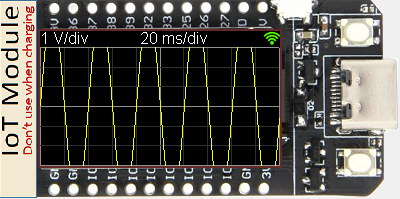
\includegraphics[width=1\linewidth]{Imagens/Testes no simulador/Vertical 1V.png}
        \captionsetup{justification=centering}
        \caption{1V/div e 20ms/div}
        \label{fig:1V/div e 20ms/div simulador}
    \end{subfigure}
    \begin{subfigure}{0.35\textwidth}
        \centering
        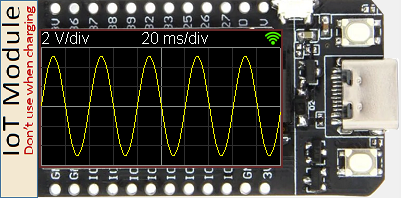
\includegraphics[width=1\linewidth]{Imagens/Testes no simulador/Vertical 2V.png}
        \captionsetup{justification=centering}
        \caption{2V/div e 20ms/div}
        \label{fig:2V/div e 20ms/div simulador}
    \end{subfigure}
    \begin{subfigure}{0.35\textwidth}
        \centering
        \includegraphics[width=1\linewidth]{Imagens/Testes no simulador/Vertical 5V.png}
        \captionsetup{justification=centering}
        \caption{5V/div e 20ms/div}
        \label{fig:5V/div e 20ms/div simulador}
    \end{subfigure}
    \begin{subfigure}{0.35\textwidth}
        \centering
        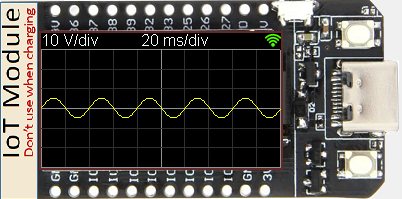
\includegraphics[width=1\linewidth]{Imagens/Testes no simulador/Vertical 10V.png}
        \captionsetup{justification=centering}
        \caption{10V/div e 20ms/div}
        \label{fig:10V/div e 20ms/div vertical simulador}
    \end{subfigure}
    \captionsetup{justification=centering}
    \caption{Variação da escala vertical (simulador)}
    \label{fig:Variação da escala vertical (simulador)}
\end{figure}

\phantom{test}

\vspace{1cm}

\begin{figure}[H]
    \centering
    \begin{subfigure}{0.35\textwidth}
        \centering
        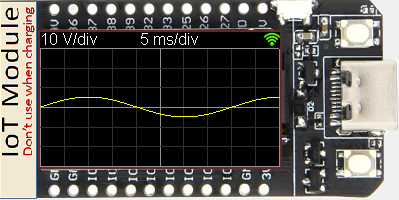
\includegraphics[width=1\linewidth]{Imagens/Testes no simulador/Horizontal 5ms.png}
        \captionsetup{justification=centering}
        \caption{10V/div e 5ms/div}
        \label{fig:10V/div e 5ms/div simulador}
    \end{subfigure}
    \begin{subfigure}{0.35\textwidth}
        \centering
        \includegraphics[width=1\linewidth]{Imagens/Testes no simulador/Horizontal 10ms.png}
        \captionsetup{justification=centering}
        \caption{10V/div e 10ms/div}
        \label{fig:10V/div e 10ms/div simulador}
    \end{subfigure}
    \begin{subfigure}{0.35\textwidth}
        \centering
        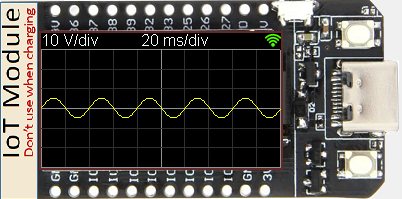
\includegraphics[width=1\linewidth]{Imagens/Testes no simulador/Horizontal 20ms.png}
        \captionsetup{justification=centering}
        \caption{10V/div e 20ms/div}
        \label{fig:10V/div e 20ms/div horizontal simulador}
    \end{subfigure}
    \begin{subfigure}{0.35\textwidth}
        \centering
        \includegraphics[width=1\linewidth]{Imagens/Testes no simulador/Horizontal 50ms.png}
        \captionsetup{justification=centering}
        \caption{10V/div e 50ms/div}
        \label{fig:10V/div e 50ms/div simulador}
    \end{subfigure}
    \captionsetup{justification=centering}
    \caption{Variação da escala horizontal (simulador)}
    \label{fig:Variação da escala horizontal (simulador)}
\end{figure}

\begin{figure}[H]
    \centering
    \includegraphics[width=0.35\textwidth]{Imagens/Testes no simulador/Botão 13.png}
    \captionsetup{justification=centering}
    \caption{Funcionamento do duplo clique do botão 1 (simulador)}
    \label{fig:Funcionamento do duplo clique do botão 1 (simulador)}
\end{figure}

\begin{figure}[H]
    \centering
    \begin{subfigure}{0.35\textwidth}
        \centering
        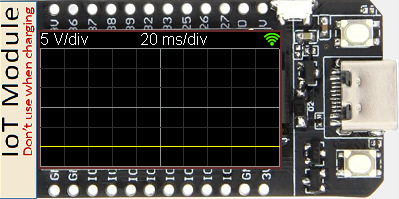
\includegraphics[width=1\linewidth]{Imagens/Testes no simulador/DC -10V.png}
        \captionsetup{justification=centering}
        \caption{DC -10V}
        \label{fig:DC -10V simulador}
    \end{subfigure}
    \begin{subfigure}{0.35\textwidth}
        \centering
        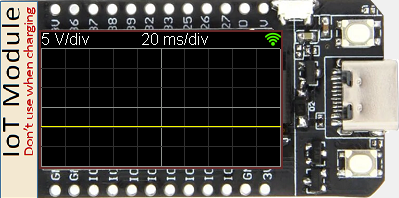
\includegraphics[width=1\linewidth]{Imagens/Testes no simulador/DC -5V.png}
        \captionsetup{justification=centering}
        \caption{DC -5V}
        \label{fig:DC -5V simulador}
    \end{subfigure}
    \begin{subfigure}{0.35\textwidth}
        \centering
        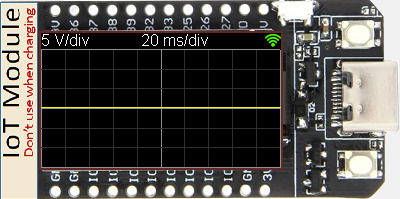
\includegraphics[width=1\linewidth]{Imagens/Testes no simulador/DC 0V.png}
        \captionsetup{justification=centering}
        \caption{DC 0V}
        \label{fig:DC 0V simulador}
    \end{subfigure}
    \begin{subfigure}{0.35\textwidth}
        \centering
        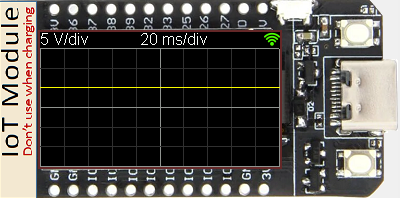
\includegraphics[width=1\linewidth]{Imagens/Testes no simulador/DC 5V.png}
        \captionsetup{justification=centering}
        \caption{DC 5V}
        \label{fig:DC 5V simulador}
    \end{subfigure}
\end{figure}

\begin{figure}[H]\ContinuedFloat
    \centering
    \begin{subfigure}{0.35\textwidth}
        \centering
        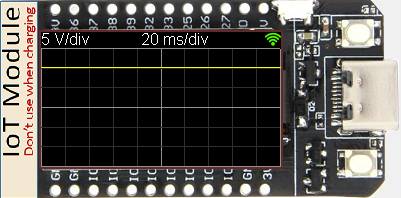
\includegraphics[width=1\linewidth]{Imagens/Testes no simulador/DC 10V.png}
        \captionsetup{justification=centering}
        \caption{DC 10V}
        \label{fig:DC 10V simulador}
    \end{subfigure}
    \captionsetup{justification=centering}
    \caption{Variação de uma tensão DC (simulador)}
    \label{fig:Variação de uma tensão DC (simulador)}
\end{figure}

Aqui não se apresenta a onda quadrada com que o programa tem de ser testado uma vez que o obtido é exatamente igual ao que está no enunciado. A funcionalidade da DFT será demonstrada nos \nameref{sec:Testes no laboratório}.

Como seria de esperar, no simulador com a calibração de origem do Professor verifica-se a correta representação de todos os sinais e funcionalidade do programa desenvolvido. Nos testes experimentais é inevitável que haja erros a nível de ruído e no conjunto de medidas determinado, o que será discutido de seguida.

\section{Testes no laboratório}\label{sec:Testes no laboratório}
    \subsection{Não calibrado}\label{subsec:Não calibrado}
        Novamente, mas agora experimentalmente, apresenta-se de seguida os resultados obtidos para um sinal sinusoidal de $25$Hz, $5$V de amplitude e $0$V de \textit{offset}, para a variação de uma fonte DC (escala de $5$V/div como pedido) e ainda uma onda quadrada de $60$Hz, $4$V de amplitude e $-1$V de \textit{offset}. Para obter estes dados sem calibração comenta-se a linha \texttt{76} e descomentam-se as linhas \texttt{73}, \texttt{74} e \texttt{75} da função \texttt{read\_and\_calculate()}.

\vspace{1cm}

\begin{figure}[H]
    \centering
    \begin{subfigure}{0.35\textwidth}
        \centering
        \includegraphics[width=1\linewidth]{Imagens/Testes no laboratório/Não calibrado/Vertical 1V.png}
        \captionsetup{justification=centering}
        \caption{1V/div e 20ms/div}
        \label{fig:1V/div e 20ms/div não calibrado}
    \end{subfigure}
    \begin{subfigure}{0.35\textwidth}
        \centering
        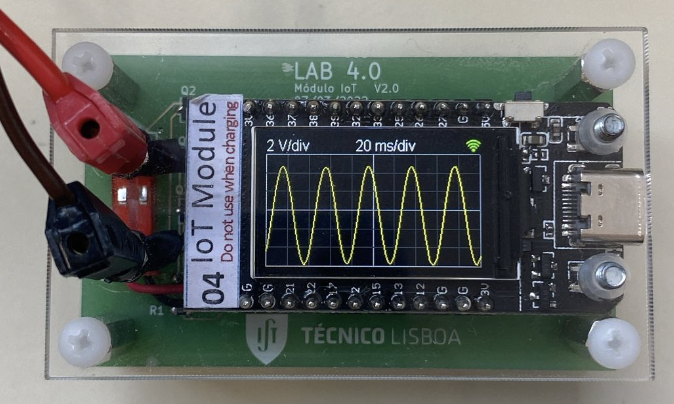
\includegraphics[width=1\linewidth]{Imagens/Testes no laboratório/Não calibrado/Vertical 2V.png}
        \captionsetup{justification=centering}
        \caption{2V/div e 20ms/div}
        \label{fig:2V/div e 20ms/div não calibrado}
    \end{subfigure}
    \begin{subfigure}{0.35\textwidth}
        \centering
        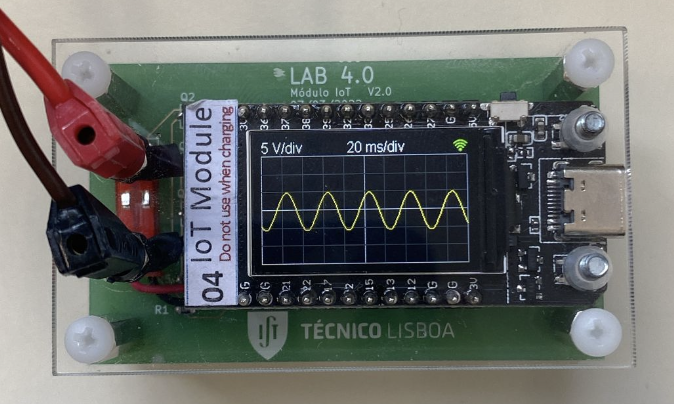
\includegraphics[width=1\linewidth]{Imagens/Testes no laboratório/Não calibrado/Vertical 5V.png}
        \captionsetup{justification=centering}
        \caption{5V/div e 20ms/div}
        \label{fig:5V/div e 20ms/div não calibrado}
    \end{subfigure}
    \begin{subfigure}{0.35\textwidth}
        \centering
        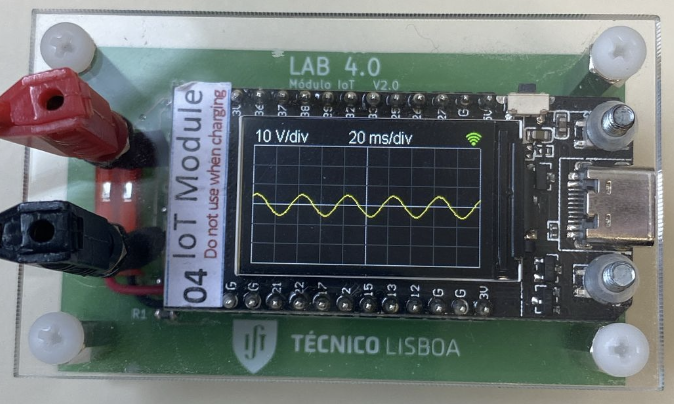
\includegraphics[width=1\linewidth]{Imagens/Testes no laboratório/Não calibrado/Vertical 10V.png}
        \captionsetup{justification=centering}
        \caption{10V/div e 20ms/div}
        \label{fig:10V/div e 20ms/div vertical não calibrado}
    \end{subfigure}
    \captionsetup{justification=centering}
    \caption{Variação da escala vertical (não calibrado)}
    \label{fig:Variação da escala vertical (não calibrado)}
\end{figure}

\begin{figure}[H]
    \centering
    \begin{subfigure}{0.35\textwidth}
        \centering
        \includegraphics[width=1\linewidth]{Imagens/Testes no laboratório/Não calibrado/Horizontal 5ms.png}
        \captionsetup{justification=centering}
        \caption{10V/div e 5ms/div}
        \label{fig:10V/div e 5ms/div não calibrado}
    \end{subfigure}
    \begin{subfigure}{0.35\textwidth}
        \centering
        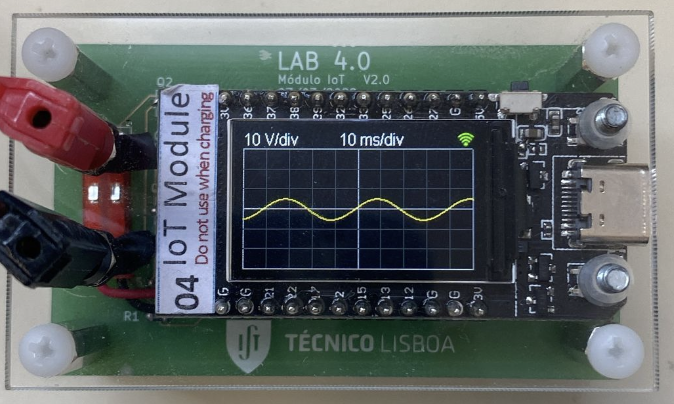
\includegraphics[width=1\linewidth]{Imagens/Testes no laboratório/Não calibrado/Horizontal 10ms.png}
        \captionsetup{justification=centering}
        \caption{10V/div e 10ms/div}
        \label{fig:10V/div e 10ms/div não calibrado}
    \end{subfigure}
    \begin{subfigure}{0.35\textwidth}
        \centering
        \includegraphics[width=1\linewidth]{Imagens/Testes no laboratório/Não calibrado/Horizontal 20ms.png}
        \captionsetup{justification=centering}
        \caption{10V/div e 20ms/div}
        \label{fig:10V/div e 20ms/div horizontal não calibrado}
    \end{subfigure}
    \begin{subfigure}{0.35\textwidth}
        \centering
        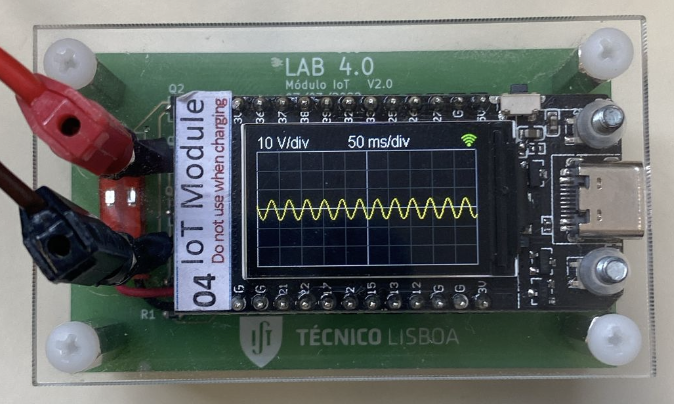
\includegraphics[width=1\linewidth]{Imagens/Testes no laboratório/Não calibrado/Horizontal 50ms.png}
        \captionsetup{justification=centering}
        \caption{10V/div e 50ms/div}
        \label{fig:10V/div e 50ms/div não calibrado}
    \end{subfigure}
    \captionsetup{justification=centering}
    \caption{Variação da escala horizontal (não calibrado)}
    \label{fig:Variação da escala horizontal (não calibrado)}
\end{figure}

\begin{figure}[H]
    \centering
    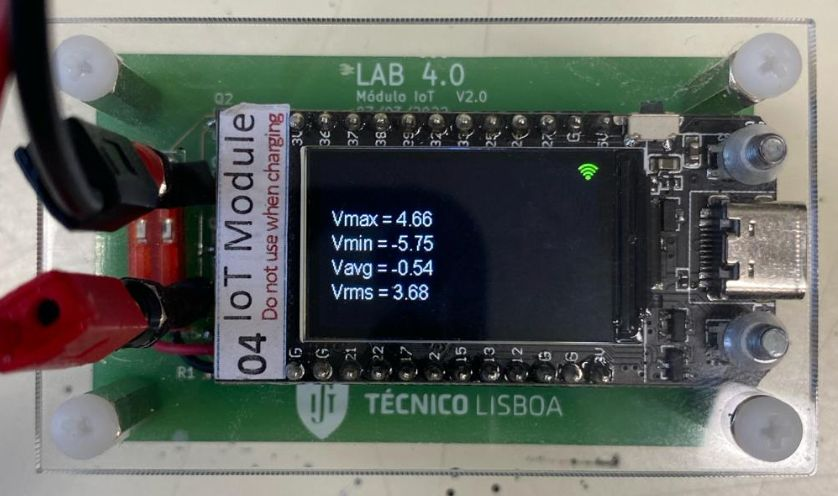
\includegraphics[width=0.35\textwidth]{Imagens/Testes no laboratório/Não calibrado/Botão 13.jpeg}
    \captionsetup{justification=centering}
    \caption{Funcionamento do duplo clique do botão 1 (não calibrado)}
    \label{fig:Funcionamento do duplo clique do botão 1 (não calibrado)}
\end{figure}

\vspace{-0.25cm}

\begin{figure}[H]
    \centering
    \begin{subfigure}{0.35\textwidth}
        \centering
        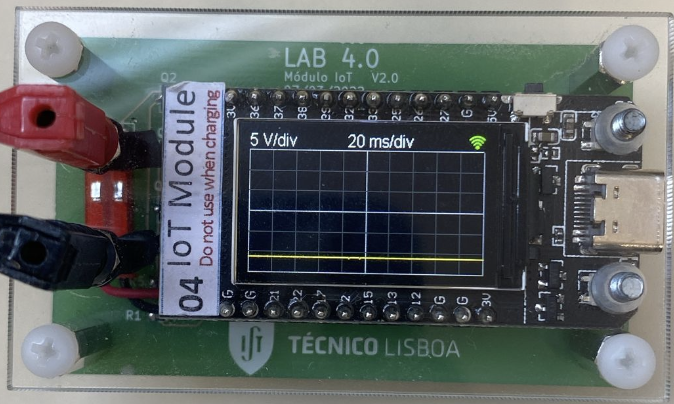
\includegraphics[width=1\linewidth]{Imagens/Testes no laboratório/Não calibrado/DC -10V.png}
        \captionsetup{justification=centering}
        \caption{DC -10V}
        \label{fig:DC -10V não calibrado}
    \end{subfigure}
    \begin{subfigure}{0.35\textwidth}
        \centering
        \includegraphics[width=1\linewidth]{Imagens/Testes no laboratório/Não calibrado/DC -5V.png}
        \captionsetup{justification=centering}
        \caption{DC -5V}
        \label{fig:DC -5V não calibrado}
    \end{subfigure}
    \begin{subfigure}{0.35\textwidth}
        \centering
        \includegraphics[width=1\linewidth]{Imagens/Testes no laboratório/Não calibrado/DC 0V.png}
        \captionsetup{justification=centering}
        \caption{DC 0V}
        \label{fig:DC 0V não calibrado}
    \end{subfigure}
    \begin{subfigure}{0.35\textwidth}
        \centering
        \includegraphics[width=1\linewidth]{Imagens/Testes no laboratório/Não calibrado/DC 5V.png}
        \captionsetup{justification=centering}
        \caption{DC 5V}
        \label{fig:DC 5V não calibrado}
    \end{subfigure}
\end{figure}

\begin{figure}[H]\ContinuedFloat
    \centering
    \begin{subfigure}{0.35\textwidth}
        \centering
        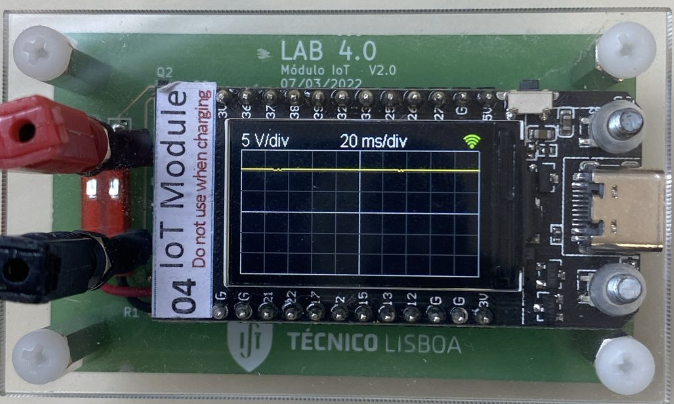
\includegraphics[width=1\linewidth]{Imagens/Testes no laboratório/Não calibrado/DC 10V.png}
        \captionsetup{justification=centering}
        \caption{DC 10V}
        \label{fig:DC 10V não calibrado}
    \end{subfigure}
    \captionsetup{justification=centering}
    \caption{Variação de uma tensão DC (não calibrado)}
    \label{fig:Variação de uma tensão DC (não calibrado)}
\end{figure}

\begin{figure}[H]
    \centering
    \begin{subfigure}{0.35\textwidth}
        \centering
        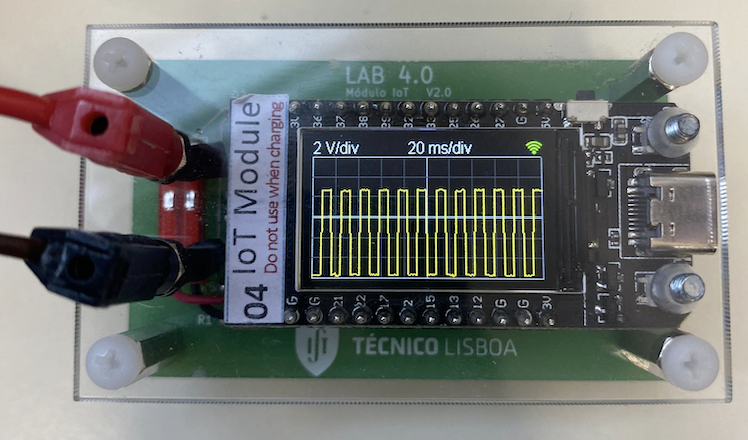
\includegraphics[width=1\linewidth]{Imagens/Testes no laboratório/Não calibrado/Onda quadrada do enunciado.png}
        \captionsetup{justification=centering}
        \caption{Onda quadrada}
        \label{fig:Onda quadrada não calibrado}
    \end{subfigure}
    \begin{subfigure}{0.35\textwidth}
        \centering
        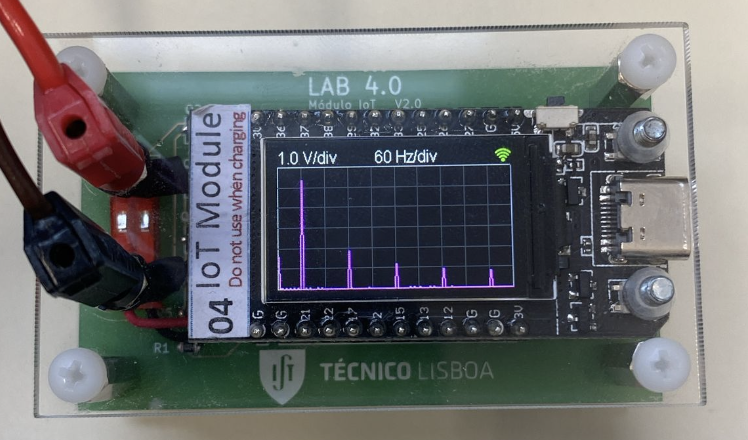
\includegraphics[width=1\linewidth]{Imagens/Testes no laboratório/Não calibrado/Onda quadrada do enunciado espetro.png}
        \captionsetup{justification=centering}
        \caption{Espetro da onda quadrada}
        \label{fig:Espetro da onda quadrada não calibrado}
    \end{subfigure}
    \captionsetup{justification=centering}
    \caption{Onda quadrada do enunciado e o seu espetro (não calibrado)}
    \label{fig:Onda quadrada do enunciado e o seu espetro (não calibrado)}
\end{figure}

Como era de esperar, verifica-se a necessidade de calibrar o sistema por mera observação das imagens acima no que toca à incorreta representação dos sinais e, nomeadamente, o erro associado ao conjunto de medidas evidenciado na \autoref{fig:Funcionamento do duplo clique do botão 1 (não calibrado)} (facilmente observável pelas tensões máxima e mínima apresentadas).
    \subsection{Ajuste experimental}\label{subsec:Ajuste experimental}
        Verificada a necessidade de efetuar a calibração, ou seja, fazer corresponder o valor digital obtido através do conversor analógico-digital ao valor de entrada do mesmo, utilizou-se o gerador de funções disponível no laboratório. Com este simulou-se uma fonte DC ao gerar um sinal com uma frequência e amplitude pico a pico praticamente nulas ($f\approx0$ e $V_{pp}\approx0$). Simulada esta fonte, alterou-se o valor do \textit{offset} na gama de valores $\{-5,-4,-3,-2,-1,0,1,2,3,4,5\}$ como é visível pelos pontos e escala das ordenadas da \autoref{fig:Reta de ajuste experimental}. 

\begin{figure}[H]
    \centering
    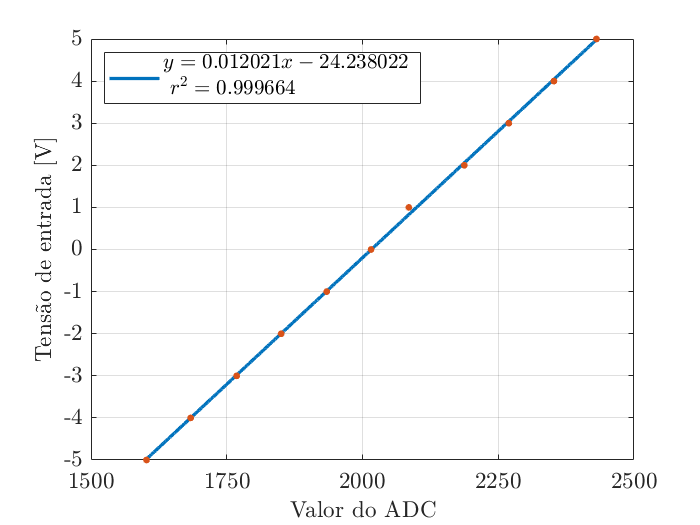
\includegraphics[width=0.47\textwidth]{Imagens/Testes no laboratório/Ajuste experimental/Calibração experimental.png}
    \captionsetup{justification=centering}
    \caption{Reta de ajuste experimental}
    \label{fig:Reta de ajuste experimental}
\end{figure}

À medida que se alteravam os valores usufruiu-se do \textit{script} \texttt{main\_exemplo\_2.py} para calcular a média de $100$ amostras cujos valores representam o eixo das abcissas da \autoref{fig:Reta de ajuste experimental}. Note-se que o gráfico acima é o inverso do apresentado no enunciado, pelo que no código da função \texttt{read\_and\_calculate()}, e já tendo a equação de ajuste, aparecem as linhas \texttt{73}, \texttt{74} e \texttt{75} comentadas e a \texttt{76} descomentada. Para confirmação do bom ajuste usou-se o \textit{script} \texttt{main\_exemplo\_1.py} com o qual se verificou que para uma tensão DC de $5$V o valor médio era $5.06$V ($\text{Erro}=1.2\%<5\%$ - indicação de bom ajuste).
    \subsection{Calibrado}\label{subsec:Calibrado}
        Como na secção anterior, apresenta-se de seguida os resultados obtidos para um sinal sinusoidal de $25$Hz, $5$V de amplitude e $0$V de \textit{offset}, para a variação de uma fonte DC (escala de $5$V/div como pedido) e ainda uma onda quadrada de $60$Hz, $4$V de amplitude e $-1$V de \textit{offset}. Agora com o ajuste experimental, comentam-se as linhas \texttt{73}, \texttt{74} e \texttt{75} e descomenta-se a linha \texttt{76} da função \texttt{read\_and\_calculate()}.

\vspace{1.5cm}

\begin{figure}[H]
    \centering
    \begin{subfigure}{0.35\textwidth}
        \centering
        \includegraphics[width=1\linewidth]{Imagens/Testes no laboratório/Calibrado/Vertical 1V.png}
        \captionsetup{justification=centering}
        \caption{1V/div e 20ms/div}
        \label{fig:1V/div e 20ms/div calibrado}
    \end{subfigure}
    \begin{subfigure}{0.35\textwidth}
        \centering
        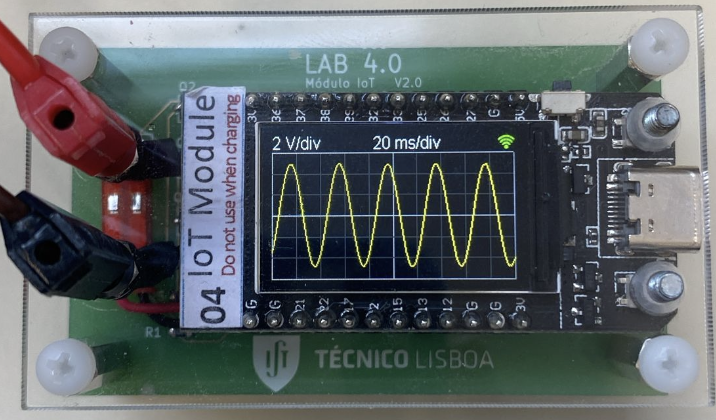
\includegraphics[width=1\linewidth]{Imagens/Testes no laboratório/Calibrado/Vertical 2V.png}
        \captionsetup{justification=centering}
        \caption{2V/div e 20ms/div}
        \label{fig:2V/div e 20ms/div calibrado}
    \end{subfigure}
    \begin{subfigure}{0.35\textwidth}
        \centering
        \includegraphics[width=1\linewidth]{Imagens/Testes no laboratório/Calibrado/Vertical 5V.png}
        \captionsetup{justification=centering}
        \caption{5V/div e 20ms/div}
        \label{fig:5V/div e 20ms/div calibrado}
    \end{subfigure}
    \begin{subfigure}{0.35\textwidth}
        \centering
        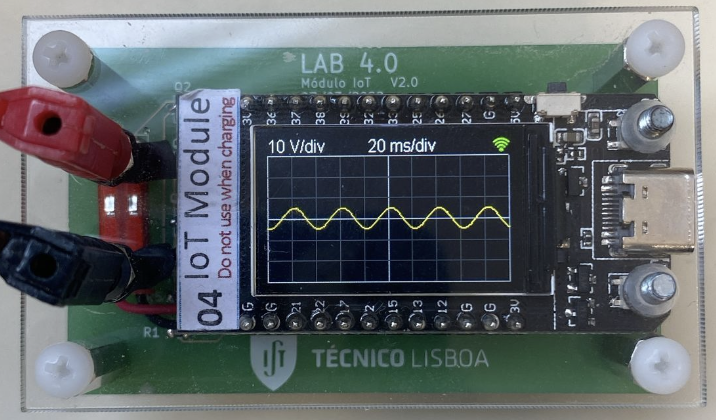
\includegraphics[width=1\linewidth]{Imagens/Testes no laboratório/Calibrado/Vertical 10V.png}
        \captionsetup{justification=centering}
        \caption{10V/div e 20ms/div}
        \label{fig:10V/div e 20ms/div vertical calibrado}
    \end{subfigure}
    \captionsetup{justification=centering}
    \caption{Variação da escala vertical (calibrado)}
    \label{fig:Variação da escala vertical (calibrado)}
\end{figure}

\begin{figure}[H]
    \centering
    \begin{subfigure}{0.35\textwidth}
        \centering
        \includegraphics[width=1\linewidth]{Imagens/Testes no laboratório/Calibrado/Horizontal 5ms.png}
        \captionsetup{justification=centering}
        \caption{10V/div e 5ms/div}
        \label{fig:10V/div e 5ms/div calibrado}
    \end{subfigure}
    \begin{subfigure}{0.35\textwidth}
        \centering
        \includegraphics[width=1\linewidth]{Imagens/Testes no laboratório/Calibrado/Horizontal 10ms.png}
        \captionsetup{justification=centering}
        \caption{10V/div e 10ms/div}
        \label{fig:10V/div e 10ms/div calibrado}
    \end{subfigure}
\end{figure}

\begin{figure}[H]\ContinuedFloat
    \centering
    \begin{subfigure}{0.35\textwidth}
        \centering
        \includegraphics[width=1\linewidth]{Imagens/Testes no laboratório/Calibrado/Horizontal 20ms.png}
        \captionsetup{justification=centering}
        \caption{10V/div e 20ms/div}
        \label{fig:10V/div e 20ms/div horizontal calibrado}
    \end{subfigure}
    \begin{subfigure}{0.35\textwidth}
        \centering
        \includegraphics[width=1\linewidth]{Imagens/Testes no laboratório/Calibrado/Horizontal 50ms.png}
        \captionsetup{justification=centering}
        \caption{10V/div e 50ms/div}
        \label{fig:10V/div e 50ms/div calibrado}
    \end{subfigure}
    \captionsetup{justification=centering}
    \caption{Variação da escala horizontal (calibrado)}
    \label{fig:Variação da escala horizontal (calibrado)}
\end{figure}

\vspace{-0.4cm}

\begin{figure}[H]
    \centering
    \includegraphics[width=0.35\textwidth]{Imagens/Testes no laboratório/Calibrado/Botão 13.jpeg}
    \captionsetup{justification=centering}
    \caption{Funcionamento do duplo clique do botão 1 (calibrado)}
    \label{fig:Funcionamento do duplo clique do botão 1 (calibrado)}
\end{figure}

\vspace{-0.4cm}

\begin{figure}[H]
    \centering
    \begin{subfigure}{0.35\textwidth}
        \centering
        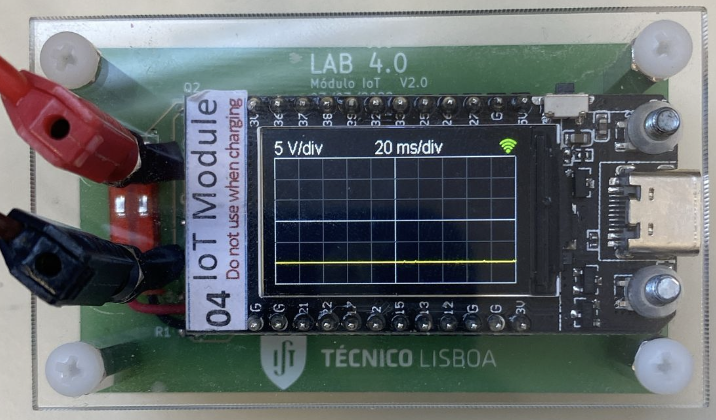
\includegraphics[width=1\linewidth]{Imagens/Testes no laboratório/Calibrado/DC -10V.png}
        \captionsetup{justification=centering}
        \caption{DC -10V}
        \label{fig:DC -10V calibrado}
    \end{subfigure}
    \begin{subfigure}{0.35\textwidth}
        \centering
        \includegraphics[width=1\linewidth]{Imagens/Testes no laboratório/Calibrado/DC -5V.png}
        \captionsetup{justification=centering}
        \caption{DC -5V}
        \label{fig:DC -5V calibrado}
    \end{subfigure}
    \begin{subfigure}{0.35\textwidth}
        \centering
        \includegraphics[width=1\linewidth]{Imagens/Testes no laboratório/Calibrado/DC 0V.png}
        \captionsetup{justification=centering}
        \caption{DC 0V}
        \label{fig:DC 0V calibrado}
    \end{subfigure}
    \begin{subfigure}{0.35\textwidth}
        \centering
        \includegraphics[width=1\linewidth]{Imagens/Testes no laboratório/Calibrado/DC 5V.png}
        \captionsetup{justification=centering}
        \caption{DC 5V}
        \label{fig:DC 5V calibrado}
    \end{subfigure}
    \begin{subfigure}{0.35\textwidth}
        \centering
        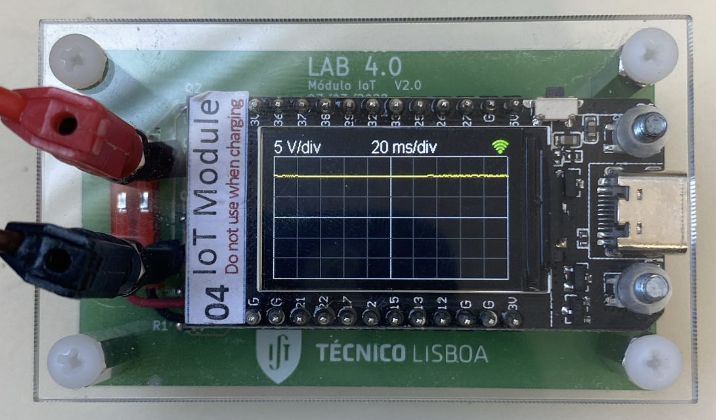
\includegraphics[width=1\linewidth]{Imagens/Testes no laboratório/Calibrado/DC 10V.png}
        \captionsetup{justification=centering}
        \caption{DC 10V}
        \label{fig:DC 10V calibrado}
    \end{subfigure}
    \captionsetup{justification=centering}
    \caption{Variação de uma tensão DC (calibrado)}
    \label{fig:Variação de uma tensão DC (calibrado)}
\end{figure}

\begin{figure}[H]
    \centering
    \begin{subfigure}{0.35\textwidth}
        \centering
        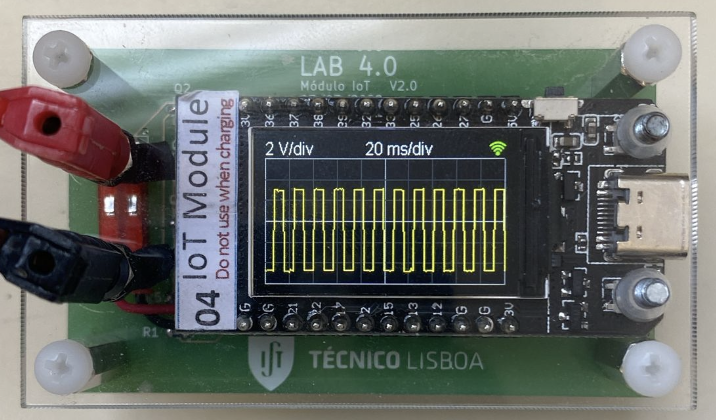
\includegraphics[width=1\linewidth]{Imagens/Testes no laboratório/Calibrado/Onda quadrada do enunciado.png}
        \captionsetup{justification=centering}
        \caption{Onda quadrada}
        \label{fig:Onda quadrada calibrado}
    \end{subfigure}
    \begin{subfigure}{0.35\textwidth}
        \centering
        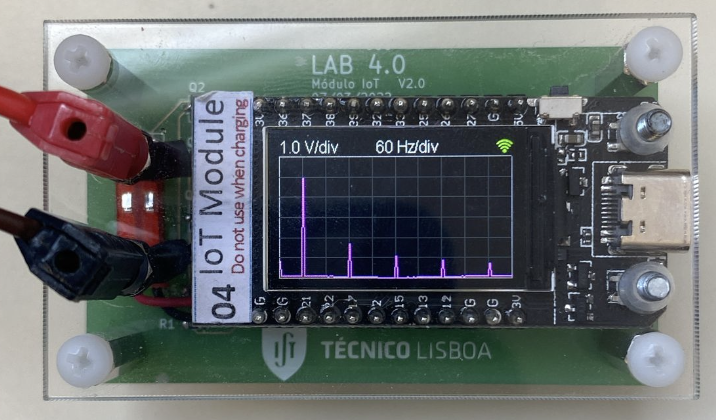
\includegraphics[width=1\linewidth]{Imagens/Testes no laboratório/Calibrado/Onda quadrada do enunciado espetro.png}
        \captionsetup{justification=centering}
        \caption{Espetro da onda quadrada}
        \label{fig:Espetro da onda quadrada calibrado}
    \end{subfigure}
    \captionsetup{justification=centering}
    \caption{Onda quadrada do enunciado e o seu espetro (calibrado)}
    \label{fig:Onda quadrada do enunciado e o seu espetro (calibrado)}
\end{figure}

Como previsto, a calibração permitiu obter representações dos sinais realmente corretas como se pode ver nas ilustrações acima apresentadas. No entanto, como dito na \nameref{sec:Introdução}, as imperfeições não são completamente aniquiladas devido às não idealidades do sistema que causam ruído (particularmente visível na \autoref{fig:Variação de uma tensão DC (calibrado)}), nomeadamente a impedância associada ao gerador de funções usado para gerar o sinal de entrada e fazer curto-circuito no módulo IoT. Pela \autoref{fig:Funcionamento do duplo clique do botão 1 (calibrado)} vemos ainda o efeito das não idealidades no cálculo de \texttt{Vmin}, uma vez que este não é o simétrico de \texttt{Vmax}. Pela \autoref{fig:Onda quadrada do enunciado e o seu espetro (calibrado)} vemos também o efeito do ruído na representação no domínio do tempo e, por sua vez, um ligeiro decréscimo do pico principal do espetro.

Desta maneira, após testes em simulação e no laboratório verifica-se o correto funcionamento do ficheiro \texttt{main.py} desenvolvido, assim como um bom ajuste experimental para o módulo IoT $04$ utilizado.

        
\section{Conclusões}\label{sec:Conclusões}
    \input{Texto/Conclusões}

% ----------------------------------------------------------------------
%                                 Bibliografia
% ----------------------------------------------------------------------
\newpage
\pagestyle{fancy}
\fancyhf{} % Limpar todos os cabeçalhos e rodapés
\renewcommand{\headrulewidth}{0pt} % Remover linha do cabeçalho
\renewcommand{\footrulewidth}{0pt} % Remover linha do rodapé
% % \renewcommand{\refname}{Bibliografia} % Alterar o título da seção de referências para "Bibliografia"
% \bibliographystyle{unsrt}
% \bibliography{refs}

% %para alterar as referências é irem ao documento refs.bib e alterar ou criar. para fazer uma referência ao longo do texto é usarem o comando \cite que está aí em cima

% ----------------------------------------------------------------------
%                                 Apêndices
% ----------------------------------------------------------------------
% \newpage
\appendix  
\addappheadtotoc 
\appendixpage

\section{Ficheiro de código desenvolvido completo}\label{ap:Ficheiro de código desenvolvido completo}
    \lstset{style=mystyle_complete_code}
\lstinputlisting[language=Python, caption={Ficheiro de código desenvolvido completo - \texttt{main.py}}, label={lst:codigocompleto}]{codigo_completo.py}


% \lstinputlisting[language=Python, caption={Ficheiro de código desenvolvido completo - \texttt{main.py}}, label={lst:pythoncode}, firstline=40, lastline=50,firstnumber=40]{codigo_completo.py}


    
\section{Funcionalidade do envio do email}\label{ap:Funcionalidade do envio do email}
    \begin{figure}[H]
    \centering
    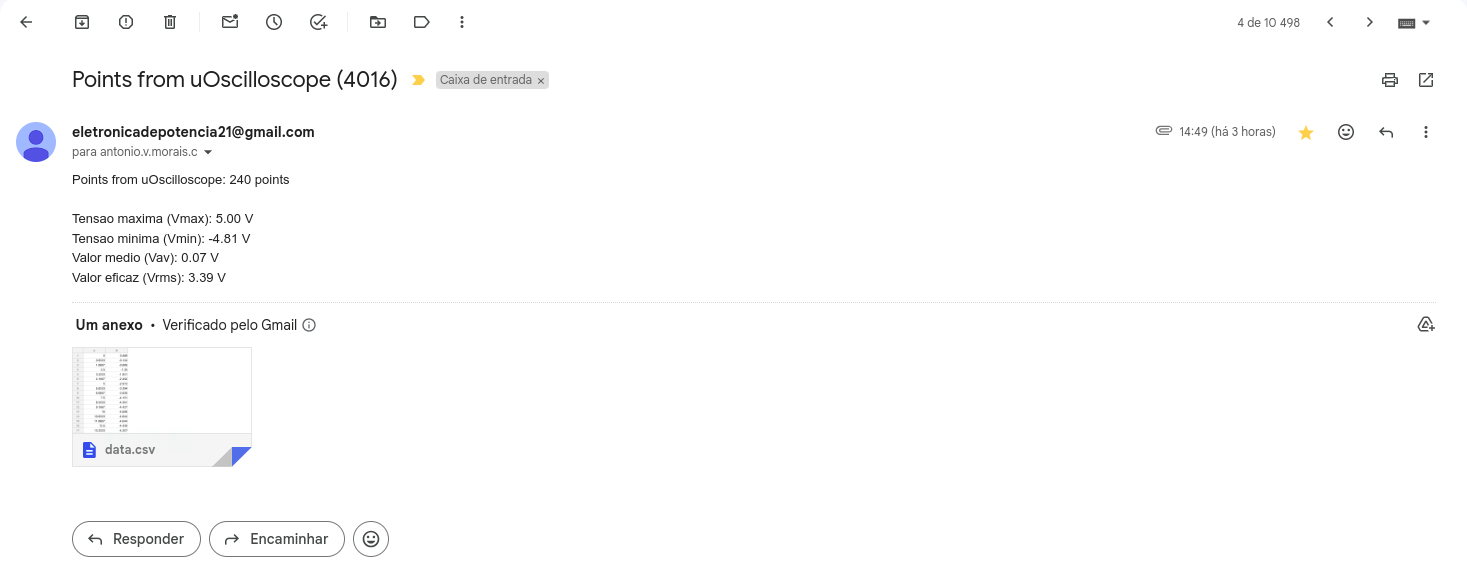
\includegraphics[width=1\textwidth]{Apêndices/Botão 12.png}
    \captionsetup{justification=centering}
    \caption{Funcionamento do clique lento do botão 1 (dados experimentais)}
    \label{fig:Funcionamento do clique lento  do botão 1 (dados experimentais)}
\end{figure}

% \newpage

% ----------------------------------------------------------------------
%                                 Anexos
% ----------------------------------------------------------------------
% \newpage
% \renewcommand{\appendixpagename}{\LARGE \fontfamily{cmss}\selectfont Anexos}
% \renewcommand{\appendixtocname}{Anexos}
% \appendix  
% \addappheadtotoc 
% \appendixpage 


% \newpage

\end{document}